\section{Numerical work}

We wish to confirm the numerical results from
\textcite{prl-selffocus}. That is, we wish to show that a Gaussian
beam is focused when propagating in a Kerr lens. Our starting point is
the full wave equation, and the assumption that the propagating beam
is cylindrical. Per \textcite{prl-selffocus} this leads to a
dimensionless form of the wave equation
\begin{align}
  \label{eq:kerr-diff}
   i \pdiff{\tilde E}{\tilde z} + \ppdiff{\tilde E}{\tilde r}
   + \frac{1}{\tilde r} \pdiff{\tilde E}{\tilde r}
   + |\tilde E|^2 \tilde E
   = 0,
\end{align}
where $\tilde r = r/a$, $a$ is a characteristic length of the beam
intensity profile, $\tilde z = z / 2ka^2$ is the characteristic axial
length of the beam, $k = n_0 \omega / c$ is the wave number of the
laser field and $\tilde E = (\chi_1/\chi_3)^{1/2} k a
\mathcal{E}$.

The point of solving the dimensionless wave equation is, that we
minimize the dependence on physical properties of the beam. This
simplifies the numerical approach and makes it easier to obtain a
solution exhibiting the correct physical behaviour albeit for at
generalized monochromatic circular Gaussian beam.

The partial differential equation given in Eqn.~\eqref{eq:kerr-diff}
is categorized as a 1D diffusion problem. To simplify notation, we
drop the tildes from the variables in the following discussion, but
the variables remain dimensionless. 
A method for solving this problem is
the Crank-Nicolson method, which applies for equations of the form
\begin{equation}
  \label{eq:Crank-Nicolson}
  \pdiff{u}{t} = F \Big(u, x, t, \pdiff{u}{x}, \ppdiff{u}{x} \Big). 
\end{equation}
This is the case for our equation, since it can be rewritten as
\begin{equation}
  \label{eq:kerr-diff-crank}
  i\pdiff{E}{z} = -\frac{1}{r} \pdiff{E}{r} - \ppdiff{E}{r} - |E|^{2} E. 
\end{equation}

In order to evaluate this numerically we discretise $z$ and $r$ in order to make a grid. The first
and second order derivatives can then be approximated by the central finite difference
\begin{equation}
  \label{eq:central-diff}
  f'(x) = \frac{f(x+\half h) - f(x - \half x)}{h} \quad f''(x) = \frac{f(x+h) - 2f(x) + f(x-h)}{h^{2}}.
\end{equation}

The Crank-Nicolson method relates the value of $E$ at the $n+1$ $z$-step to the value in the
$n$'th step via the equalities of the forward and backward Euler method. Note that $i$ denote the
step in $r$
\begin{equation}
  \label{eq:Crank-Nicolson-discrete}
  \frac{E^{n+1}_{i} - E^{n}_{i}}{\Delta z} = \half \big[F_{i}^{n+1}+F_{i}^{n} \big].
\end{equation}
The right hand side of the can be evaluated using the central difference approximation. This gives
a set of equations for $E^{n+1}$ that depends on $E^{n}$ i.e. the values in the previous step
\begin{align}
  \notag
  (\alpha + 2\beta^{2} - |E_{i}^{n+1}|^{2})E_{i}^{n+1} - \beta^{2}(E_{i+2}^{n+1} + E_{i-2}^{n+1}) -
  \frac{\beta}{r_{i}} (E_{i+1}^{n+1} - E_{i-1}^{n+1}) \\
  = (\alpha - 2\beta^{2} + |E_{i}^{n}|^{2})E_{i}^{n} + \beta^{2}(E_{i+2}^{n} + E_{i-2}^{n}) +
  \frac{\beta}{r_{i}} (E_{i+1}^{n} - E_{i-1}^{n}), 
  \label{eq:kerr-long}
\end{align}
where $\alpha = -2i/\!{\Delta z}$ and $\beta = 1/{2 \Delta r}$.

This is almost a five-diagonal matrix equation except for the term that is cubic in
$E_{i}^{n+1}$. However with sufficiently small steps one can approximate the cubic term so that
$|E_{i}^{n+1}|^{2}E_{i}^{n+1} \approx |E_{i}^{n}|^{2}E_{i}^{n+1}$ i.e. take the quadratic part from
the last step. In each time step, one must then solve the matrix inversion problem
\begin{equation}
  \label{eq:matrix}
  \mathbf{A} \mathbf{E}^{n+1} = \mathbf{B} \mathbf{E}^{n}, 
\end{equation}
where the coefficients that make up these two matrices are the coefficients listed in
Eqn.~\eqref{eq:kerr-long}. 

\subsection{Results}
\label{sec:kerr-results}

We have implemented the Crank-Nicolson algorithm in the Python language. The source code can be found at
\url{https://github.com/Munken/Laser}.

For the numerical simulation, the boundary conditions are quite important. Since our beam is Gaussian,
we enforce that $E \rightarrow 0$ as $r \rightarrow \infty$.
Furthermore the first derivative in $r = 0$ should be 0 since the beam is cylindrically symmetric.

We have tried to introduce these boundary conditions in two ways. \Cref{fig:kerr-double} shows a
simulation where we have simulated on $\pm r$. \Cref{fig:kerr-single} shows the same simulation
where we have only simulated from 0. It is clear from these two figures that we have numerical
instabilities for the small $r$-values. We have not been able to solve this problem so we have not
been able to reproduce \cite{prl-selffocus}[Fig. 1]. 
\begin{figure}[htb]
  \centering
  \subbottom[Symmetric\label{fig:kerr-double}]{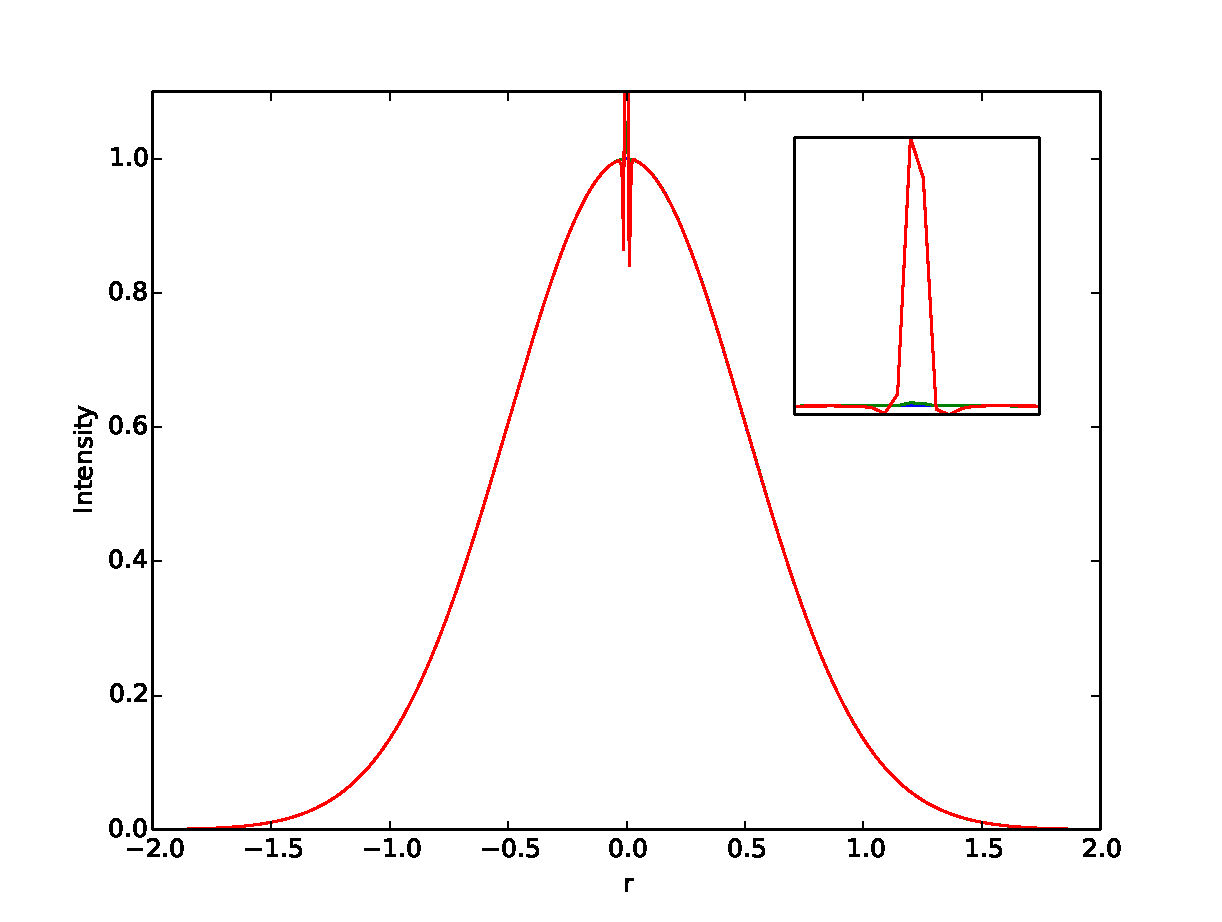
\includegraphics[width=0.45\columnwidth]{kerr_double}}
  \hfill
  \subbottom[Symmetric\label{fig:kerr-single}]{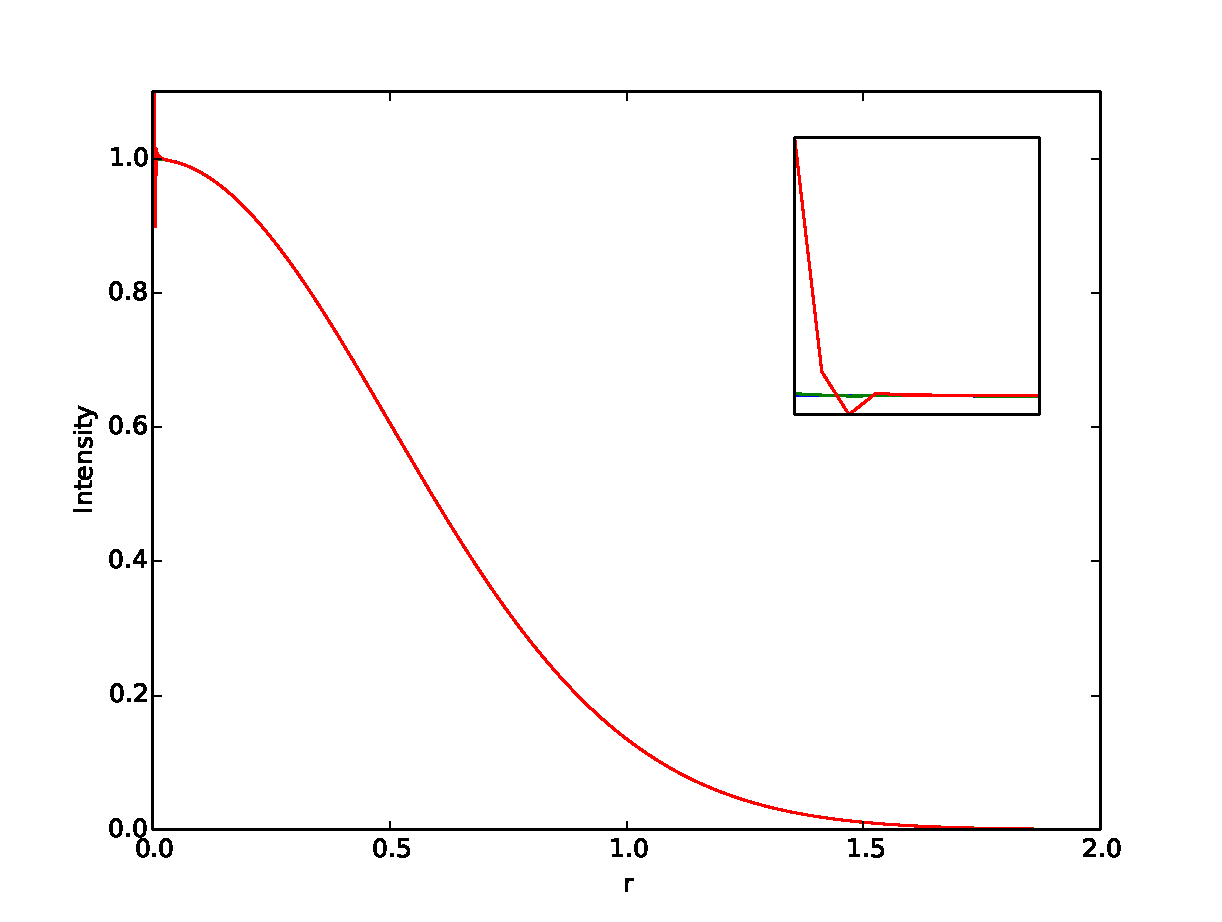
\includegraphics[width=0.45\columnwidth]{kerr_single}}
  \caption{The result of our numerical simulation after propagating 10 steps. The insets shows the
    behaviour around $r=0$.}
  \label{fig:kerr-num}
\end{figure}



%%% Local Variables: 
%%% mode: latex
%%% TeX-master: "nonlinear"
%%% End: 
